% adapted by WS from SSR's Word document and from the 5-part series at
% https://www.overleaf.com/learn/latex/How_to_Write_a_Thesis_in_LaTeX_(Part_1):_Basic_Structure
% reviewed by MAM

\documentclass[12pt,twosided]{report}

\usepackage[titletoc]{appendix} % for adding appendix to TOC
\usepackage{biblatex}  % reference management
\usepackage{geometry}  % better margins and margin control
\usepackage{graphicx}  % to include figures
\usepackage{hyperref}  % internal and external links
\usepackage[utf8]{inputenc}  % support for non-ASCII characters
\usepackage{listings}  % typset code
\usepackage{outlines}  % easy nesting of lists
\usepackage{tabularx}  % more control over table column width
\usepackage{titlesec}  % customize chapter title 
\usepackage{upquote}  % prevent mishandling of single quotes in listings


% TODO: Customize the appearance of hyperref links using \hypersetup
% See https://en.wikibooks.org/wiki/LaTeX/Hyperlinks#Customization

% Custom format of chapter title.
\titleformat{\chapter}[hang]{\bf\huge}{\thechapter.}{2pc}{}

% Separate folder for images named 'images'.
\graphicspath{ {images/} }

% Separate file for references
\addbibresource{references.bib}

% Replace with your title
\title{The COVID-19 Pandemic: A Biological Insight Using Augmented Reality}

% Allow recalling document title
% from https://tex.stackexchange.com/a/15806/44301
\makeatletter\let\Title\@title\makeatother  

\begin{document}

\begin{titlepage}
  
  \newgeometry{top=100pt,bottom=75pt}   
  \begin{center}
    \vfill
    \textbf{\Huge \Title}
    \bigskip

    {\large Kaavish Report\\
      presented to the academic faculty\\
      by\\\bigskip
      % replace with your name and HU ID
      \begin{tabular}{ll}
        Owais Bin Asad & oa05007\\
        Aaron Lucas Soares & as04345\\
        Arham Ahmed & aa05179\\
      \end{tabular}
    }\\\vfill
    \includegraphics[width=.4\textwidth]{logo.pdf}\\
    {\large In partial fulfillment of the requirements for\\
      \textit{Bachelor of Science}\\
      Computer Science\\\medskip
      \textbf{Dhanani School of Science and Engineering}\\\medskip
      Habib University\\\smallskip
      Spring 2022
    }\\\vfill
    Copyright {\scriptsize \textcopyright} 2019 Habib University
  \end{center}
  \restoregeometry
\end{titlepage}

%%% Local Variables:
%%% mode: latex
%%% TeX-master: "report"
%%% End:
  % title page.
\include{approval}  % approval page.

\chapter*{Dedication}
TBD.

\chapter*{Acknowledgements}
TBD.

\chapter*{Abstract}
Abstract goes here

% The following are automatically populated by LaTeX \chapter, \section and related, \figure, and \table.
\tableofcontents
\listoffigures
\listoftables

\chapter{Introduction}
\label{chap:intro}
\section{Problem Statement}
Towards the end of 2019, a novel virus emerged and spread throughout the city of Wuhan in China. A few months later, on 11th March 2020, the World Health Organization (WHO) officially declared that the SARS-CoV-2 virus has caused a global pandemic. Nearly two years later, the Covid-19 virus still poses a threat to humanity despite the countless efforts to thwart its spread and eliminate the virus through vaccinations. To this day, our general understanding of viruses is quite limited as people fail to understand how viruses infect humans and how they could potentially cause epidemics and pandemics by spreading through infected individuals. In our project, we aim to educate students about what viruses are, how they infect humans and how they can cause epidemics and pandemics.

\section{Proposed Solution}
In order to understand the mechanisms of the SARS-CoV-2 virus and how to prepare ourselves for future epidemics/pandemics, we plan on educating the population, especially students, about what a virus is, how it works, how it spreads, and its ability to mutate to ensure its survival through an AR platform. This will be done using an ecosystem of interactive models, games, and simulations in AR to ensure that the students don’t just learn for the sake of school but because their curiosity is peaked.

\section{Intended User}
Middle School and High School students who have access to a smartphone and internet.

\section{Project gantt chart and deliverables}
\subsection{Gantt Chart}
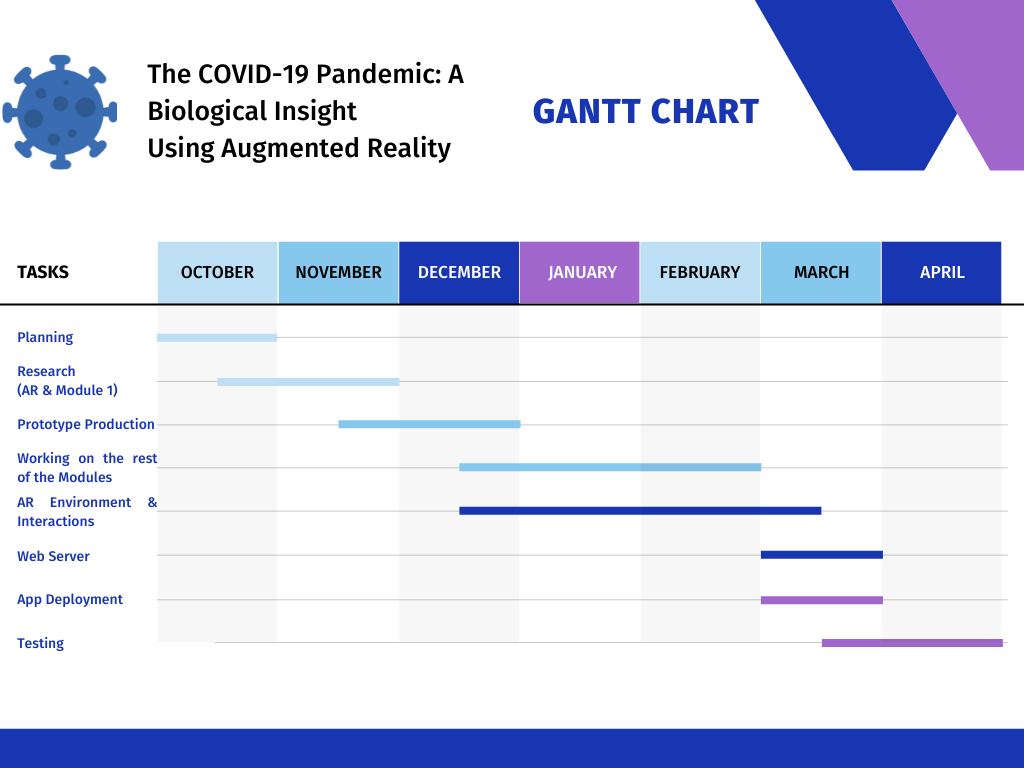
\includegraphics[scale=0.5]{ganttChart.png}

\subsection{Deliverables}
\begin{enumerate}
    \item Physical booklet to access the content 
    \item Mobile application with all the AR games and simulations
\end{enumerate}


\section{Key Challenges}
The main challenge for the team is to learn AR as it is something that we’re new to. However, given the multiple resources available online, the team will be able to learn a sufficient amount on the subject for this project. Apart from this, our project will encounter certain hardware limitations. We currently do not possess any Apple devices. Therefore the team has decided to first develop the app for Android and move on to iOS if time permits.

\chapter{Literature Review}
\label{chap:lit}
\input{chapters/review}

\chapter{Software Requirement Specification (SRS)}
\label{chap:srs}
This chapter provides detailed specifications of the system under development.

\section{Functional Requirements}
\begin{outline}
  \1 Authorization / Authentication:
  \2 To allow the user to sign up using the QR code provided in the booklet.
  \2 To allow the user to keep record of their progress to the cloud.
  \2 To allow the user to fetch progress data from the cloud each time the app starts.
  \1 Augmented Reality:
  \2 To identify physical markers from the booklet.
  \2 To render 3D models, simulations, and games on top of the identified markers.
  \2 To take touch input as a means of interaction between the user and the simulations/models.
\end{outline}

% --- The above is to be modified as per your project, e.g. a flat list if your system has limited functional requirements.

\section{Non-functional Requirements}
\begin{outline}
  \1 Performance:
  \2 The app should be able to smoothly render 3D models and simulations, ideally, without lag.
  \2 There should be minimal lag in the user interacting using touch and the model / simulation responding to it.
  \1 Availability:
  \2 The app should be readily available on compatible platform-specific app store(s).
  \1 Deployment:
  \2 The app should be deployed on an app store that ensures reliable public access.
\end{outline}

\section{External Interfaces}
\subsection{User Interfaces}
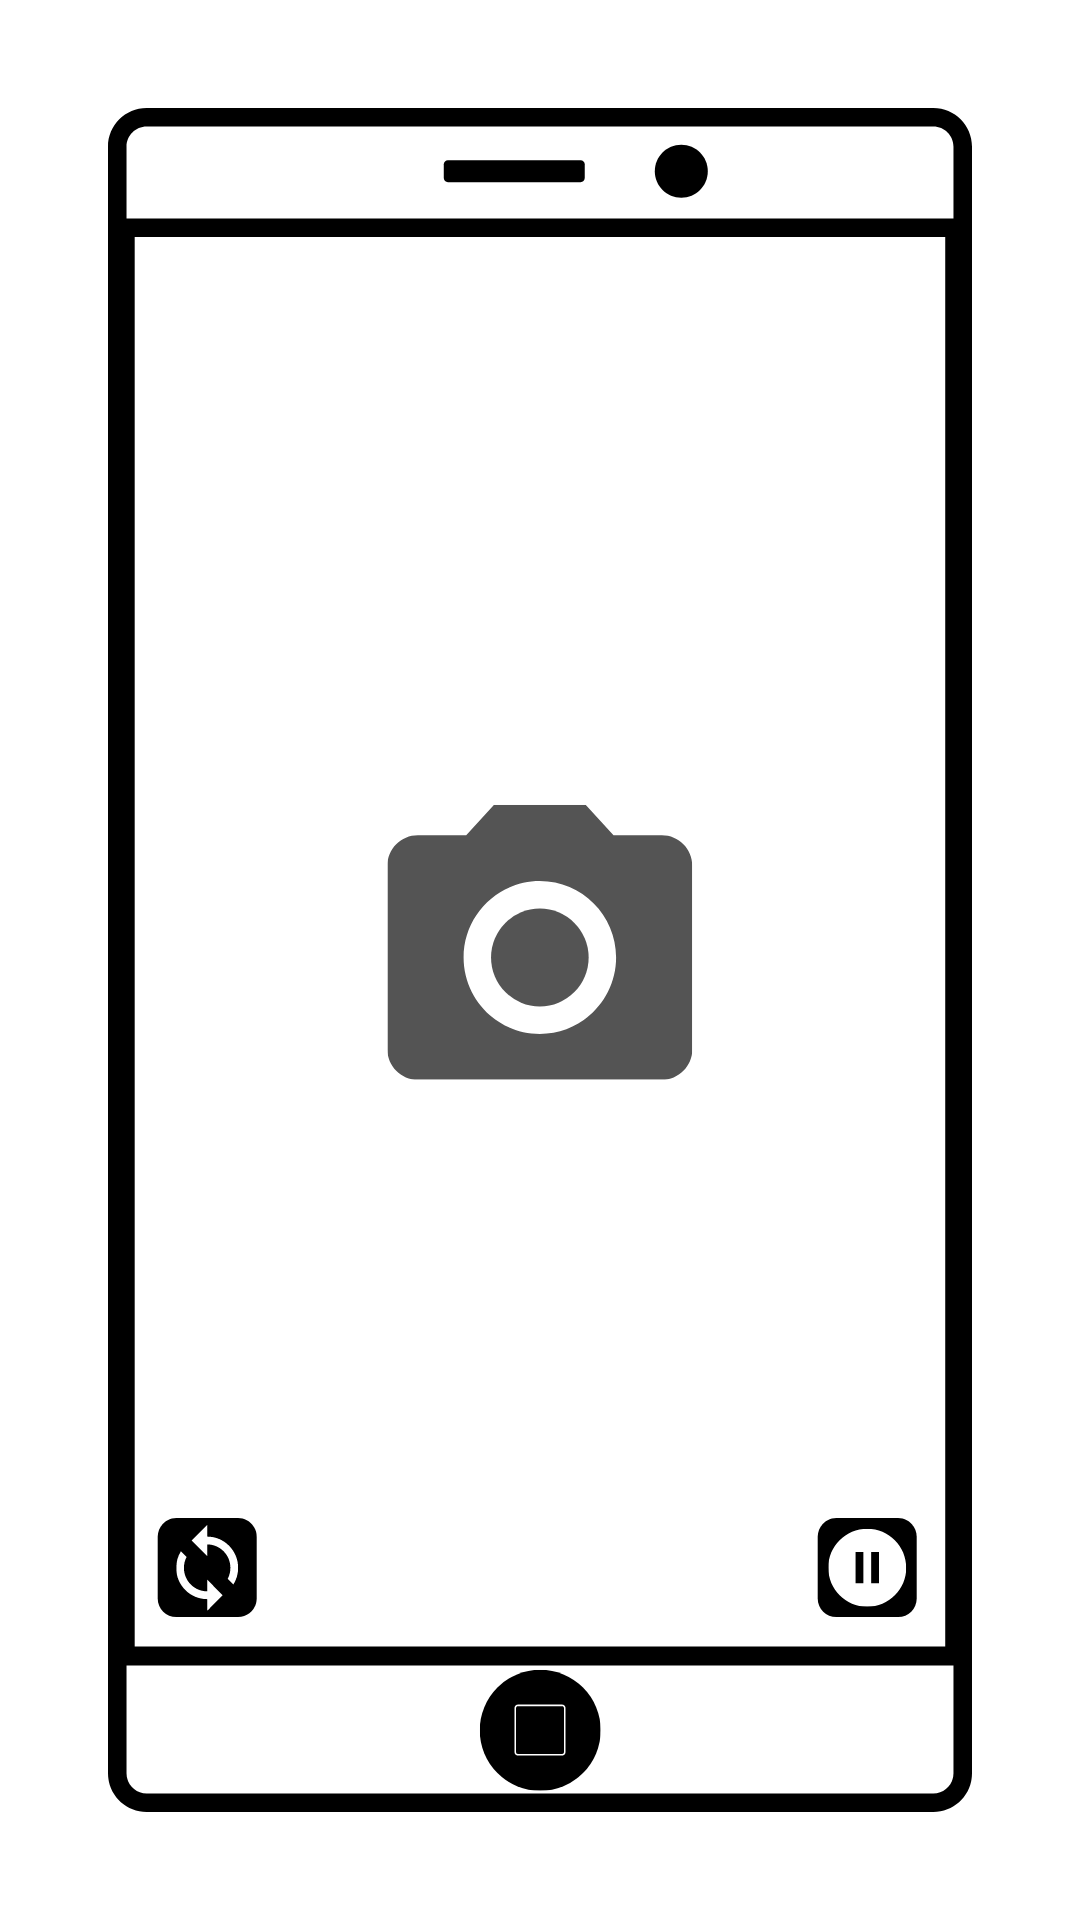
\includegraphics[scale=0.25]{appMockup.png}
\newline
Our application will deliver all of its content through AR, therefore, the mockup can only depict what the AR viewport will look like.

\section{Use Cases}
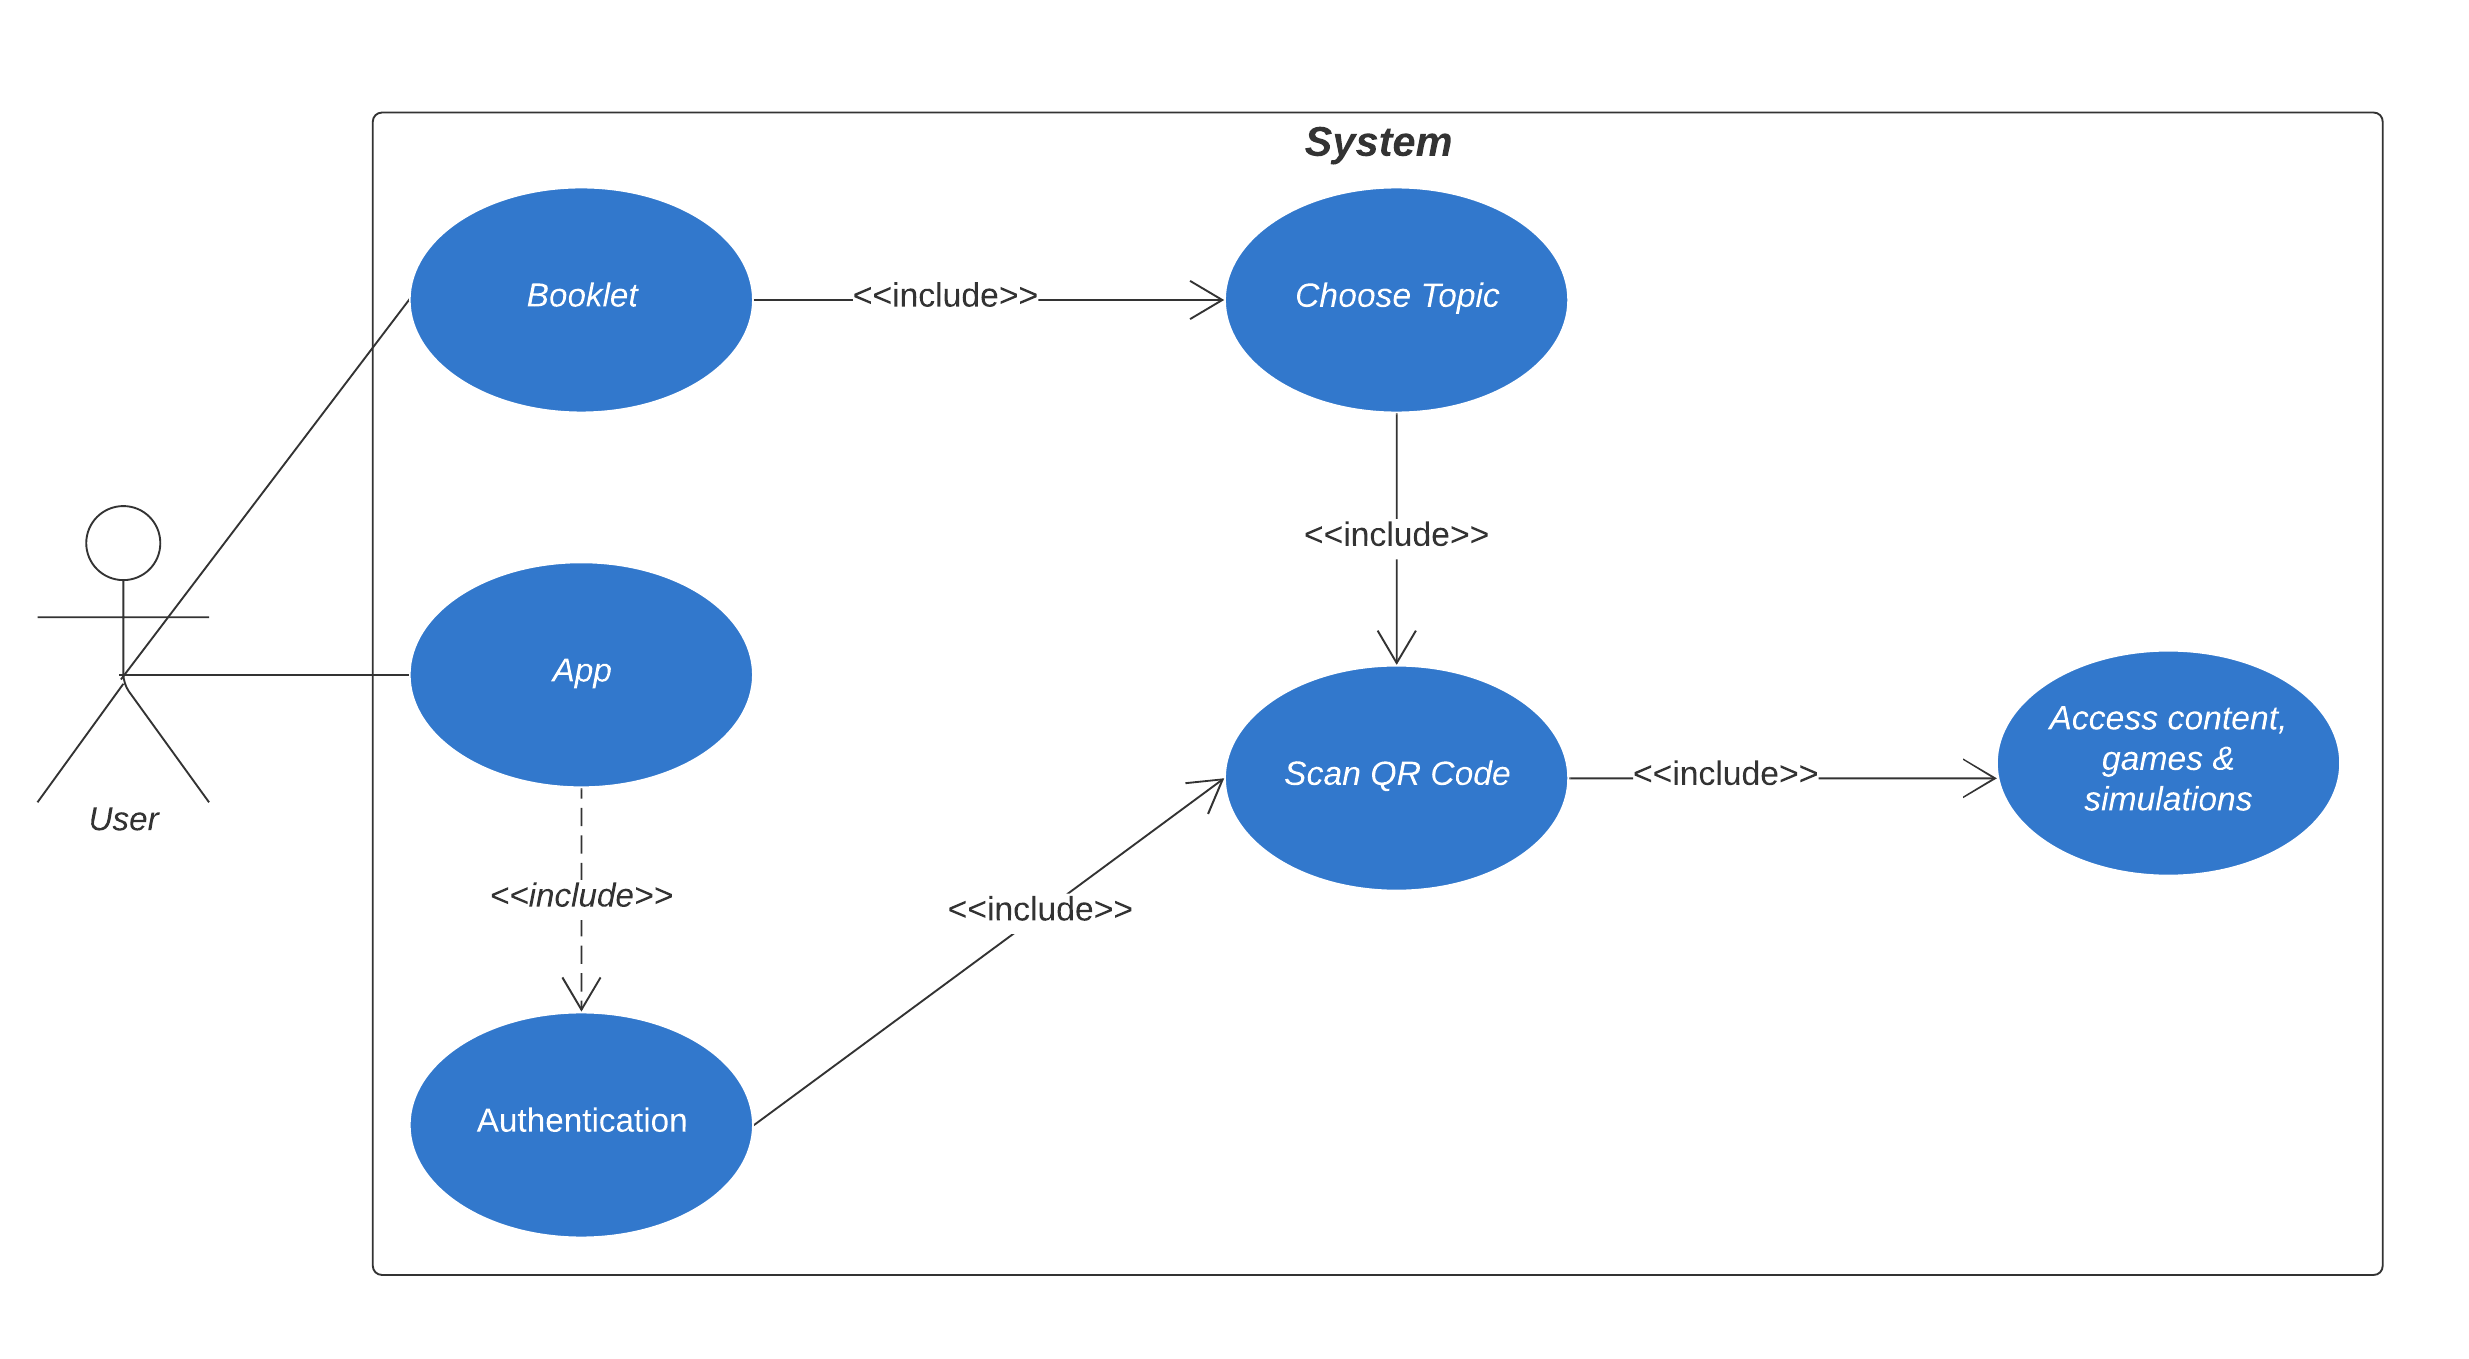
\includegraphics[scale=0.75]{useCaseDiagram.png}

\section{Datasets}
Not Applicable.

\section{System Diagram}
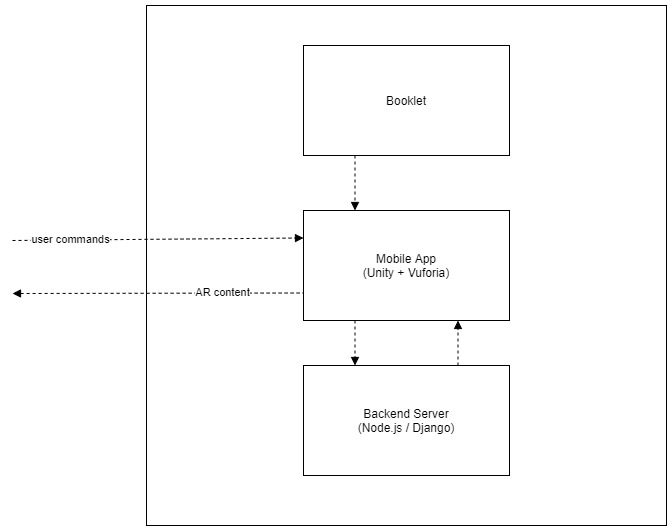
\includegraphics[scale=0.6]{systemDiagram.png}

\chapter{Software Design Specification (SDS)}
\label{chap:sds}
\input{chapters/sds}

\chapter{Experiments and Results}
\label{chap:results}
\input{chapters/results}

\chapter{Conclusion and Future Work}
\label{chap:outro}
\input{chapters/conclusion}

\begin{appendices}

\titleformat{\chapter}[hang]{\bf\huge}{Appendix \thechapter.}{2pc}{}
  
% This appendix is optional.
\chapter{More Math}
\input{chapters/appendix-math}

% This appendix is required if the data set is not fully described in the main text.
\chapter{Data}
\input{chapters/appendix-data}

% This appendix is required if the code is not fully described in the main text.
\chapter{Code}
\input{chapters/appendix-code}
\end{appendices}

% Print the bibliography with a ToC entry and titled, "References".
\printbibliography[heading=bibintoc,title={References}]

\end{document}

%%% Local Variables:
%%% mode: latex
%%% TeX-master: t
%%% End:
